\documentclass[]{article}
\usepackage{lmodern}
\usepackage{amssymb,amsmath}
\usepackage{ifxetex,ifluatex}
\usepackage{fixltx2e} % provides \textsubscript
\ifnum 0\ifxetex 1\fi\ifluatex 1\fi=0 % if pdftex
  \usepackage[T1]{fontenc}
  \usepackage[utf8]{inputenc}
\else % if luatex or xelatex
  \ifxetex
    \usepackage{mathspec}
  \else
    \usepackage{fontspec}
  \fi
  \defaultfontfeatures{Ligatures=TeX,Scale=MatchLowercase}
\fi
% use upquote if available, for straight quotes in verbatim environments
\IfFileExists{upquote.sty}{\usepackage{upquote}}{}
% use microtype if available
\IfFileExists{microtype.sty}{%
\usepackage{microtype}
\UseMicrotypeSet[protrusion]{basicmath} % disable protrusion for tt fonts
}{}
\usepackage[margin=1in]{geometry}
\usepackage{hyperref}
\hypersetup{unicode=true,
            pdftitle={Report: Hybrid vigor in response to Eimeria in the HMHZ},
            pdfauthor={Alice},
            pdfborder={0 0 0},
            breaklinks=true}
\urlstyle{same}  % don't use monospace font for urls
\usepackage{longtable,booktabs}
\usepackage{graphicx,grffile}
\makeatletter
\def\maxwidth{\ifdim\Gin@nat@width>\linewidth\linewidth\else\Gin@nat@width\fi}
\def\maxheight{\ifdim\Gin@nat@height>\textheight\textheight\else\Gin@nat@height\fi}
\makeatother
% Scale images if necessary, so that they will not overflow the page
% margins by default, and it is still possible to overwrite the defaults
% using explicit options in \includegraphics[width, height, ...]{}
\setkeys{Gin}{width=\maxwidth,height=\maxheight,keepaspectratio}
\IfFileExists{parskip.sty}{%
\usepackage{parskip}
}{% else
\setlength{\parindent}{0pt}
\setlength{\parskip}{6pt plus 2pt minus 1pt}
}
\setlength{\emergencystretch}{3em}  % prevent overfull lines
\providecommand{\tightlist}{%
  \setlength{\itemsep}{0pt}\setlength{\parskip}{0pt}}
\setcounter{secnumdepth}{0}
% Redefines (sub)paragraphs to behave more like sections
\ifx\paragraph\undefined\else
\let\oldparagraph\paragraph
\renewcommand{\paragraph}[1]{\oldparagraph{#1}\mbox{}}
\fi
\ifx\subparagraph\undefined\else
\let\oldsubparagraph\subparagraph
\renewcommand{\subparagraph}[1]{\oldsubparagraph{#1}\mbox{}}
\fi

%%% Use protect on footnotes to avoid problems with footnotes in titles
\let\rmarkdownfootnote\footnote%
\def\footnote{\protect\rmarkdownfootnote}

%%% Change title format to be more compact
\usepackage{titling}

% Create subtitle command for use in maketitle
\newcommand{\subtitle}[1]{
  \posttitle{
    \begin{center}\large#1\end{center}
    }
}

\setlength{\droptitle}{-2em}
  \title{Report: Hybrid vigor in response to Eimeria in the HMHZ}
  \pretitle{\vspace{\droptitle}\centering\huge}
  \posttitle{\par}
  \author{Alice}
  \preauthor{\centering\large\emph}
  \postauthor{\par}
  \predate{\centering\large\emph}
  \postdate{\par}
  \date{19 September 2018}

\usepackage{float} 
\let\origfigure\figure 
\let\endorigfigure\endfigure 
\renewenvironment{figure}[1][2] { 
    \expandafter\origfigure\expandafter[H] 
} { 
    \endorigfigure 
}

\begin{document}
\maketitle

{
\setcounter{tocdepth}{4}
\tableofcontents
}
\section{Eimeria detection oocysts
flotation}\label{eimeria-detection-oocysts-flotation}

\subsection{Improving Eimeria oocysts
detection}\label{improving-eimeria-oocysts-detection}

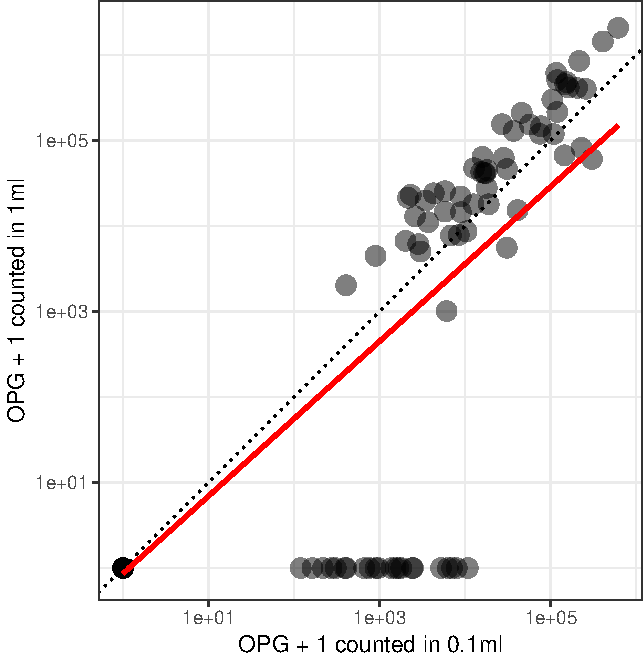
\includegraphics{Data_Analysis_Alice_files/figure-latex/oocystsDetec-1.pdf}

22 new samples were detected while diluting by 0.1mL PBS instead of 1mL
before counting in Neubauer chamber.

Adjusted R-squared = 0.81 represents the amount of variation in y
explained by x.

\subsection{OPG that we keep}\label{opg-that-we-keep}

Number of Mus musculus caught with OPG values: 486

\begin{verbatim}
## `geom_smooth()` using method = 'loess'
\end{verbatim}

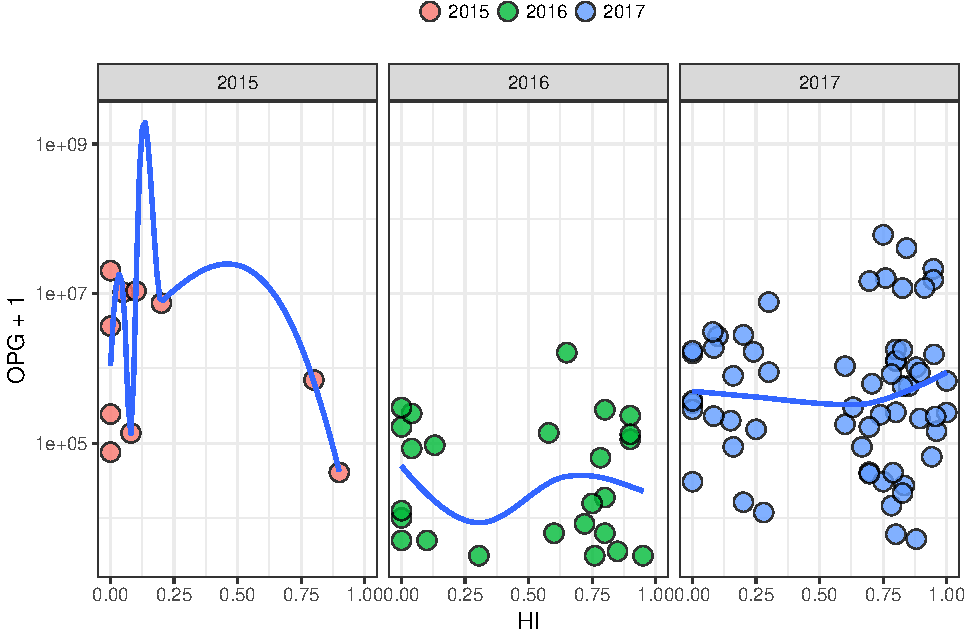
\includegraphics{Data_Analysis_Alice_files/figure-latex/oocystssmooth-1.pdf}

\section{Eimeria detection PCR}\label{eimeria-detection-pcr}

PCR positive = one of the 3 other markers than AP5 sequenced (Ap5 was
used for detection only, the other markers for confirmation)

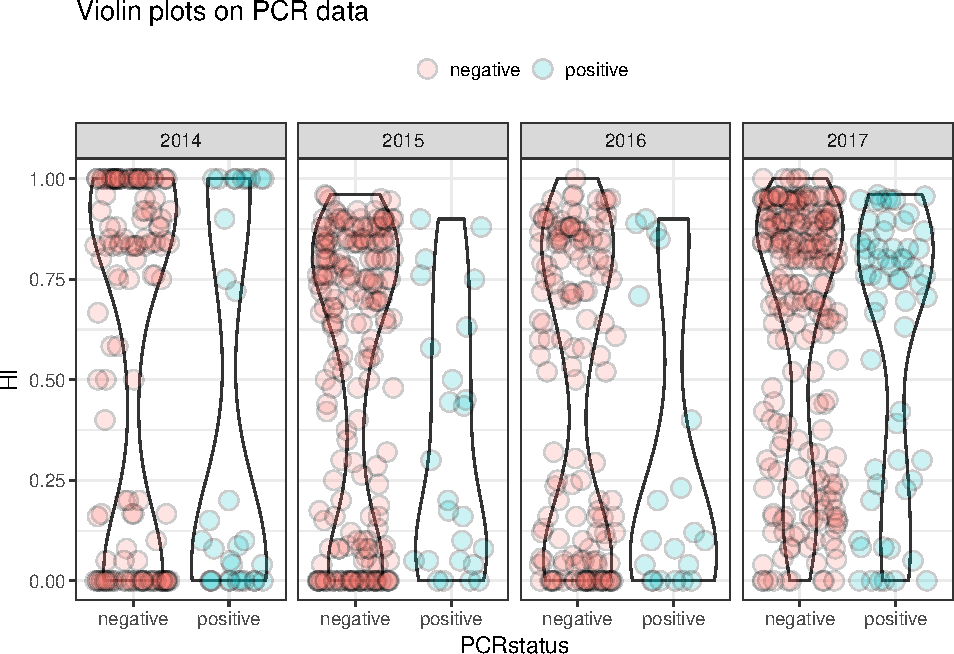
\includegraphics{Data_Analysis_Alice_files/figure-latex/pcr-1.pdf}

PCR positive = one of the 3 markers 18S, COI or ORF470) gave a sequence.
Number of Mus musculus caught with PCR performed: 962

\section{Eimeria detection qPCR}\label{eimeria-detection-qpcr}

We keep only the values for mice having been tested for BOTH ileum and
cecum!

\begin{verbatim}
## `geom_smooth()` using method = 'loess'
\end{verbatim}

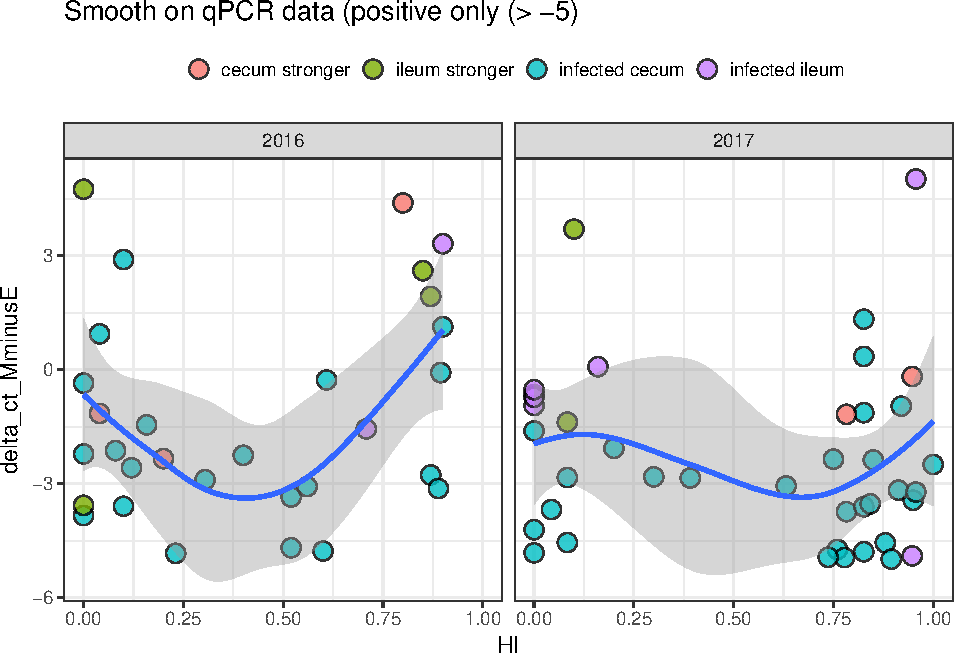
\includegraphics{Data_Analysis_Alice_files/figure-latex/qpcr-1.pdf}

\begin{verbatim}
## Warning: Removed 168 rows containing missing values (geom_point).
\end{verbatim}

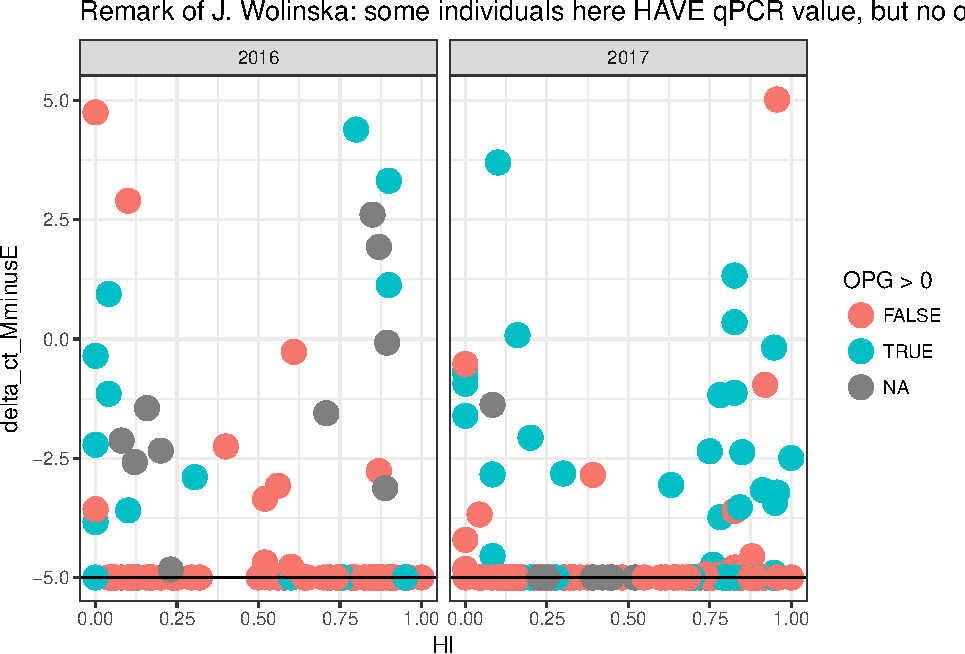
\includegraphics{Data_Analysis_Alice_files/figure-latex/qpcr-2.pdf}

Number of Mus musculus caught with qPCR performed: 371

\section{General stats on sampling}\label{general-stats-on-sampling}

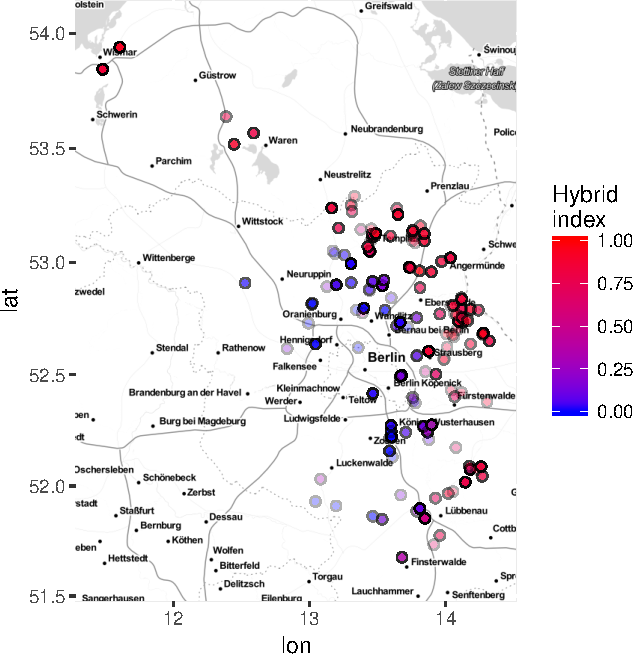
\includegraphics{Data_Analysis_Alice_files/figure-latex/generalstats-1.pdf}

We keep mice with OPG, PCR or qPCR status, in North Germany.

\begin{itemize}
\item
  Number of Mus musculus caught with OPG counted: 485
\item
  Number of Mus musculus caught with qPCR performed: 371
\item
  Number of Mus musculus caught with either OPG counted or qPCR
  performed: 513
\item
  Number of Mus musculus caught with OPG counted AND qPCR performed: 343
\item
  Some information regarding latitude and longitude are missing for the
  following mice:
\end{itemize}

SK\_3174

\begin{itemize}
\tightlist
\item
  We still miss info (HI) on the following mice (ask Jarda):
\end{itemize}

AA\_0411, AA\_0412, AA\_0420, SK\_2668, SK\_2669, SK\_2671, SK\_2674,
SK\_2675, SK\_2676, SK\_2677, SK\_2678, SK\_2681, SK\_2682, SK\_2684,
SK\_2685, SK\_2687, SK\_2688, SK\_2690, SK\_2692, SK\_2693, SK\_2695,
SK\_2696, SK\_2699, SK\_2700, SK\_2701, SK\_2702, SK\_2703, SK\_2704,
SK\_2705, SK\_2710, SK\_2713, SK\_2715, SK\_2724, SK\_2727, SK\_2729,
SK\_2733, SK\_2734, SK\_2736, SK\_2737, SK\_2738, SK\_2739, SK\_2745,
SK\_2750, SK\_2751, SK\_2752, SK\_2754, SK\_2755, SK\_2756, SK\_2758,
SK\_2759, SK\_2760, SK\_2761, SK\_2775, SK\_2778, SK\_2780, SK\_2782,
SK\_2789, SK\_2792, SK\_2793, SK\_2794, SK\_2795, SK\_2798, SK\_2799,
SK\_2800, SK\_2801, SK\_2802, SK\_2803, SK\_2804, SK\_2805, SK\_3174

\section{General informations on
HMHZ}\label{general-informations-on-hmhz}

\begin{itemize}
\item
  655 mice were captured over three years, from 157 farms
\item
  From these mice:
\item
  485 mice had Eimeria detected by feces flotation,
\item
  652 mice had Eimeria detected by colon content PCR (cf paper Victor),
\item
  371 mice had Eimeria detected by qPCR on intestinal tissues
\item
  On average, 4.04 mice were caught per farm (95\% CI 0.34)
\item
  \textbf{Hybrid indexes} were calculated as ratio of M.m.d/M.m.m
  alleles (between 4 and 14, on average 13 loci)
\end{itemize}

\begin{figure}[htbp]
\centering
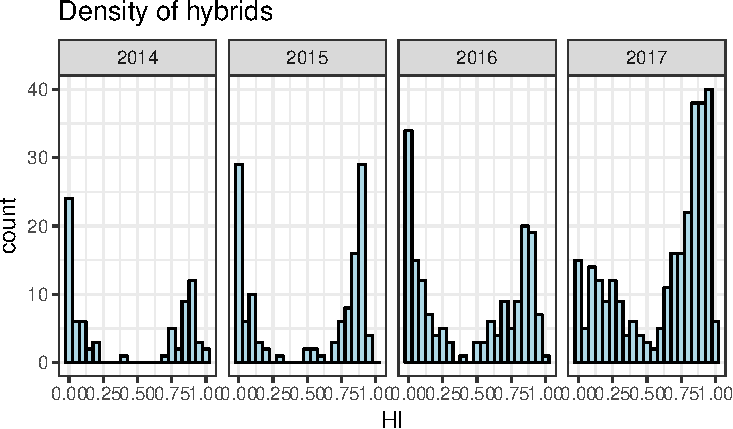
\includegraphics{Data_Analysis_Alice_files/figure-latex/plotDensHI-1.pdf}
\caption{\label{fig:plot1}Number of animals caught along the hybrid
index}
\end{figure}

\section{Prevalence of our 3 different
methods}\label{prevalence-of-our-3-different-methods}

\subsection{Prevalence tables}\label{prevalence-tables}

\begin{longtable}[]{@{}lrrrr@{}}
\caption{Prevalence of Eimeria per year, based on oocyst
flotation}\tabularnewline
\toprule
& 2014 & 2015 & 2016 & 2017\tabularnewline
\midrule
\endfirsthead
\toprule
& 2014 & 2015 & 2016 & 2017\tabularnewline
\midrule
\endhead
FALSE & 0 & 92.0 & 126.00 & 167.00\tabularnewline
TRUE & 0 & 10.0 & 25.00 & 65.00\tabularnewline
total & 0 & 102.0 & 151.00 & 232.00\tabularnewline
prevalence(\%) & NaN & 9.8 & 16.56 & 28.02\tabularnewline
\bottomrule
\end{longtable}

\begin{longtable}[]{@{}lrrrr@{}}
\caption{Prevalence of Eimeria per year, based on PCR detection. A mouse
was considered infected by Eimeria ifone of the 3 markers (COI, 18S or
ORF470) gave a sequence}\tabularnewline
\toprule
& 2014 & 2015 & 2016 & 2017\tabularnewline
\midrule
\endfirsthead
\toprule
& 2014 & 2015 & 2016 & 2017\tabularnewline
\midrule
\endhead
negative & 53.00 & 110.00 & 146.00 & 226.00\tabularnewline
positive & 23.00 & 12.00 & 20.00 & 62.00\tabularnewline
total & 76.00 & 122.00 & 166.00 & 288.00\tabularnewline
prevalence(\%) & 30.26 & 9.84 & 12.05 & 21.53\tabularnewline
\bottomrule
\end{longtable}

\begin{longtable}[]{@{}lrrrr@{}}
\caption{Prevalence of Eimeria per year, based on qPCR}\tabularnewline
\toprule
& 2014 & 2015 & 2016 & 2017\tabularnewline
\midrule
\endfirsthead
\toprule
& 2014 & 2015 & 2016 & 2017\tabularnewline
\midrule
\endhead
negative & 0 & 0 & 131.00 & 160.00\tabularnewline
positive & 0 & 0 & 33.00 & 47.00\tabularnewline
total & 0 & 0 & 164.00 & 207.00\tabularnewline
prevalence(\%) & NaN & NaN & 20.12 & 22.71\tabularnewline
\bottomrule
\end{longtable}

\begin{longtable}[]{@{}lrrrr@{}}
\caption{Prevalence of Eimeria per year, based on all detections
methods. A mouse was considered infected by Eimeria if one of the 3
markers (COI, 18S or ORF470) gave a sequence, OR if it had a positive
count of oocysts in its feces, OR if it was qPCR
positive}\tabularnewline
\toprule
& 2014 & 2015 & 2016 & 2017\tabularnewline
\midrule
\endfirsthead
\toprule
& 2014 & 2015 & 2016 & 2017\tabularnewline
\midrule
\endhead
negative & 53.00 & 105.00 & 119.00 & 193.00\tabularnewline
positive & 23.00 & 17.00 & 48.00 & 97.00\tabularnewline
total & 76.00 & 122.00 & 167.00 & 290.00\tabularnewline
prevalence(\%) & 30.26 & 13.93 & 28.74 & 33.45\tabularnewline
\bottomrule
\end{longtable}

\subsection{OPG-PCR}\label{opg-pcr}

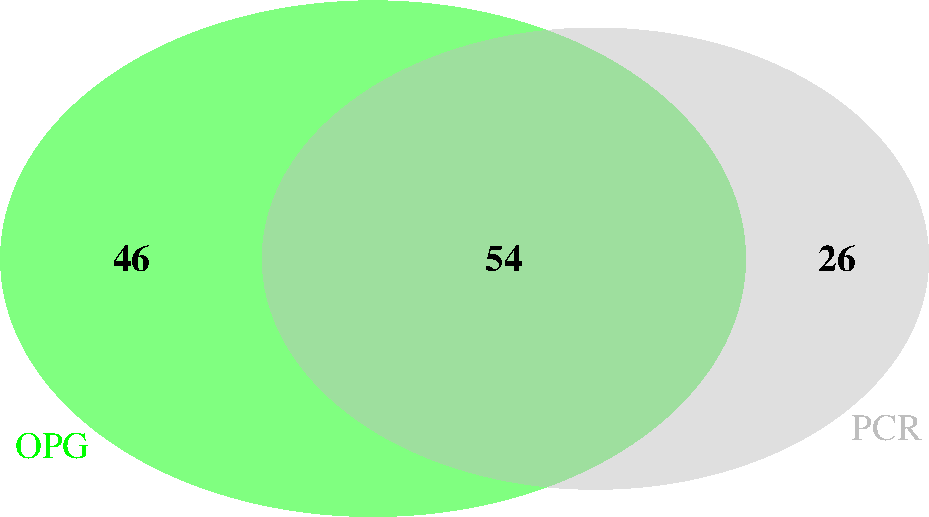
\includegraphics{Data_Analysis_Alice_files/figure-latex/opgpcr-1.pdf}

\begin{verbatim}
## (polygon[GRID.polygon.805], polygon[GRID.polygon.806], polygon[GRID.polygon.807], polygon[GRID.polygon.808], text[GRID.text.809], text[GRID.text.810], text[GRID.text.811], text[GRID.text.812], text[GRID.text.813])
\end{verbatim}

\subsection{OPG-qPCR}\label{opg-qpcr}

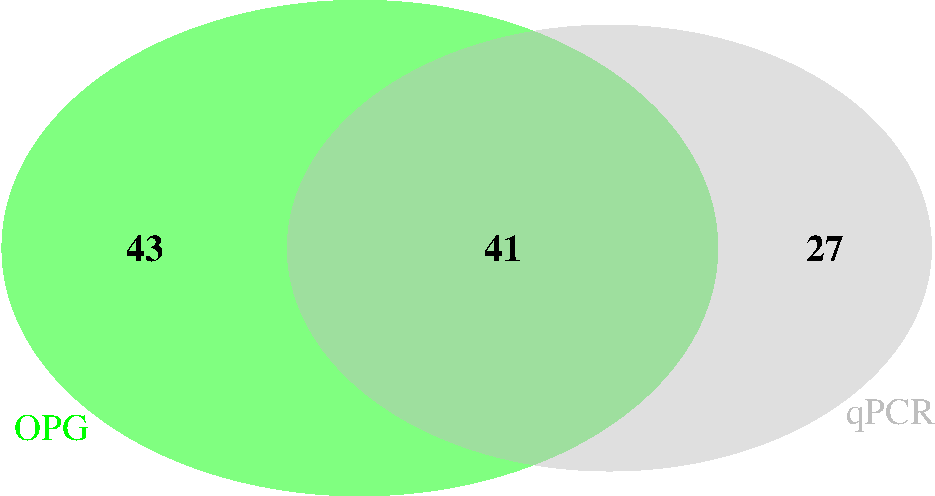
\includegraphics{Data_Analysis_Alice_files/figure-latex/opgpcrVenn-1.pdf}

\begin{verbatim}
## (polygon[GRID.polygon.814], polygon[GRID.polygon.815], polygon[GRID.polygon.816], polygon[GRID.polygon.817], text[GRID.text.818], text[GRID.text.819], text[GRID.text.820], text[GRID.text.821], text[GRID.text.822])
\end{verbatim}

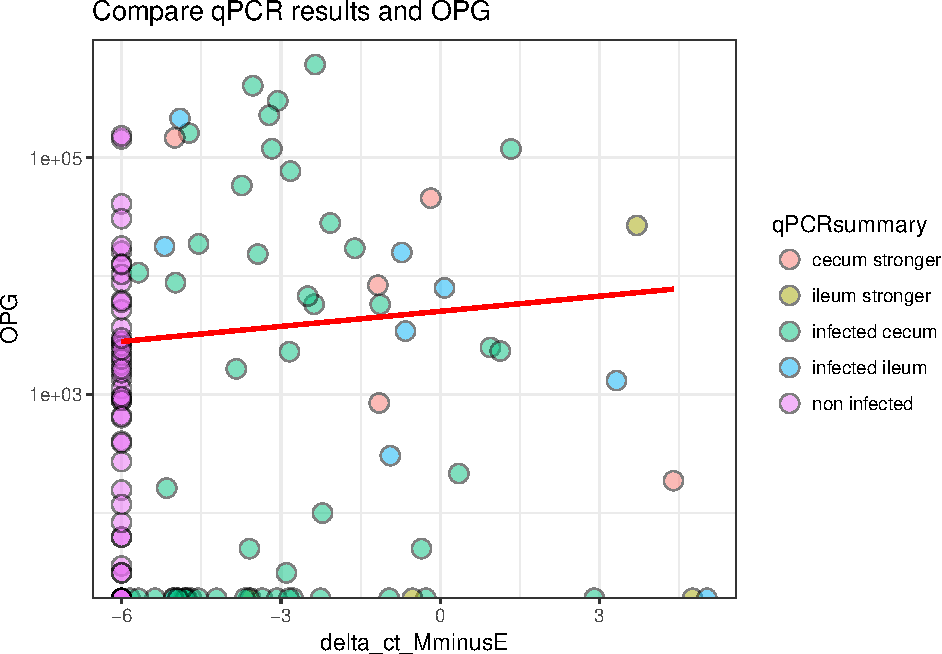
\includegraphics{Data_Analysis_Alice_files/figure-latex/opgqpcr-1.pdf}

\begin{verbatim}
## 
## Call:
## lm(formula = data1$OPG ~ data1$delta_ct_MminusE)
## 
## Residuals:
##    Min     1Q Median     3Q    Max 
## -57721  -5929  -5929  -5929 589440 
## 
## Coefficients:
##                        Estimate Std. Error t value Pr(>|t|)    
## (Intercept)               34128       7818   4.365 1.68e-05 ***
## data1$delta_ct_MminusE     4700       1395   3.368 0.000843 ***
## ---
## Signif. codes:  0 '***' 0.001 '**' 0.01 '*' 0.05 '.' 0.1 ' ' 1
## 
## Residual standard error: 48800 on 341 degrees of freedom
## Multiple R-squared:  0.0322, Adjusted R-squared:  0.02936 
## F-statistic: 11.35 on 1 and 341 DF,  p-value: 0.0008429
\end{verbatim}

\begin{verbatim}
## 
## Call:
## lm(formula = data2$OPG ~ data2$delta_ct_MminusE)
## 
## Residuals:
##     Min      1Q  Median      3Q     Max 
## -102183  -67339  -39204    6991  542133 
## 
## Coefficients:
##                        Estimate Std. Error t value Pr(>|t|)  
## (Intercept)               43423      25002   1.737   0.0903 .
## data2$delta_ct_MminusE   -11441       7946  -1.440   0.1579  
## ---
## Signif. codes:  0 '***' 0.001 '**' 0.01 '*' 0.05 '.' 0.1 ' ' 1
## 
## Residual standard error: 125100 on 39 degrees of freedom
## Multiple R-squared:  0.05048,    Adjusted R-squared:  0.02613 
## F-statistic: 2.073 on 1 and 39 DF,  p-value: 0.1579
\end{verbatim}

\subsection{OPG-qPCR-PCR}\label{opg-qpcr-pcr}

\begin{figure}[htbp]
\centering
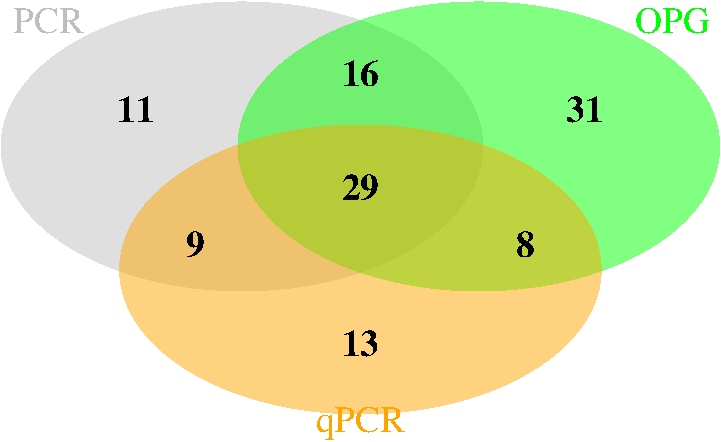
\includegraphics{Data_Analysis_Alice_files/figure-latex/venn2-1.pdf}
\caption{\label{fig:venn1}Comparison of detection: PCR vs flotation vs
qPCŔ}
\end{figure}

\begin{verbatim}
## (polygon[GRID.polygon.900], polygon[GRID.polygon.901], polygon[GRID.polygon.902], polygon[GRID.polygon.903], polygon[GRID.polygon.904], polygon[GRID.polygon.905], text[GRID.text.906], text[GRID.text.907], text[GRID.text.908], text[GRID.text.909], text[GRID.text.910], text[GRID.text.911], text[GRID.text.912], text[GRID.text.913], text[GRID.text.914], text[GRID.text.915])
\end{verbatim}

\section{BCI}\label{bci}

\subsection{BCI vs OPG}\label{bci-vs-opg}

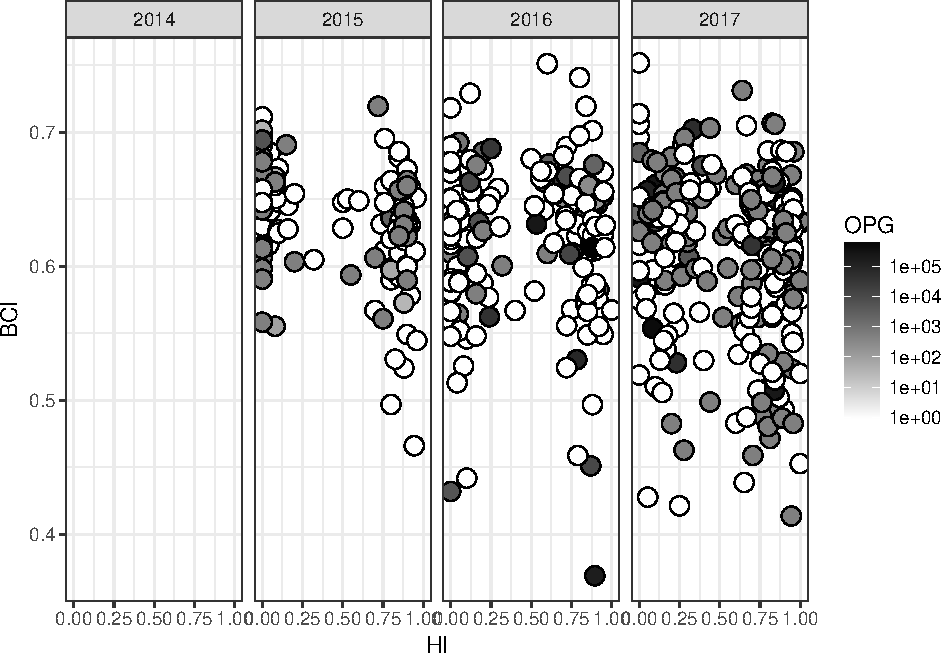
\includegraphics{Data_Analysis_Alice_files/figure-latex/BCI-1.pdf}

\begin{verbatim}
## 
## Call:
## lm(formula = myData$BCI ~ myData$OPG + myData$HI)
## 
## Residuals:
##      Min       1Q   Median       3Q      Max 
## -0.20165 -0.02542  0.01057  0.03494  0.13137 
## 
## Coefficients:
##               Estimate Std. Error t value Pr(>|t|)    
## (Intercept)  6.304e-01  4.424e-03 142.490  < 2e-16 ***
## myData$OPG  -2.061e-07  5.449e-08  -3.782 0.000176 ***
## myData$HI   -1.760e-02  6.779e-03  -2.596 0.009710 ** 
## ---
## Signif. codes:  0 '***' 0.001 '**' 0.01 '*' 0.05 '.' 0.1 ' ' 1
## 
## Residual standard error: 0.05359 on 476 degrees of freedom
##   (176 observations deleted due to missingness)
## Multiple R-squared:  0.04528,    Adjusted R-squared:  0.04127 
## F-statistic: 11.29 on 2 and 476 DF,  p-value: 1.625e-05
\end{verbatim}

\section{Testing hybrid vigor along
HMHZ}\label{testing-hybrid-vigor-along-hmhz}

\subsection{Oocyst shedding}\label{oocyst-shedding}

Statistical model (dvp\ldots{})

\subsection{qPCR proxy}\label{qpcr-proxy}

tbc

\subsection{BCI proxy}\label{bci-proxy}

tbc

\section{Bonus part: genotyping of mice
case/control}\label{bonus-part-genotyping-of-mice-casecontrol}

\begin{itemize}
\item
  100 out of 483 are positive for flotation and have an hybrid index.
\item
  80 out of 369 are positive for qPCR and have an hybrid index.
\end{itemize}

Discussed with Stuart:

\begin{itemize}
\tightlist
\item
  Test distributions 0 or counts. Test all vs only infected
  (``intensity'') distribution. We should be able to fit the
  distribution of infected on all. Zeros are data. Stochastic move.
\item
  Separation of the zero class. balanced design case/control
  \textasciitilde{} 400 +/-70infectés SNPchip.
\item
  H0: no differences are observed
\item
  Separate \textless{}0.5 and \textgreater{}0.5 to see the species
  effect
\item
  timing : WHEN (for my thesis?)
\end{itemize}


\end{document}
